\section{\textbf{Applications with AME}}

\subsection{Design}

We apply AME to three recent IR studies: \citet{reiter:stam:2003, mcdonald:2004,  weeks:2012, gibler:2017}. Each of these studies use relational data of state interactions and propose both dyadic, monadic, and structural explanations for behavior of actors in the system. We choose to demonstrate the capabilities of AME with reference to existing studies in order to highlight several features of the AME approach. First, we show that simply by using the AME framework scholars can better model the data generating process behind their events of interest. Second, the results of AME estimation are interpretable alongside results using standard approaches, but, as shown in the simulation section, have the additional benefit of being able to take into account dependencies that may otherwise complicate inference. Third, through using this approach, we can also quantify the degree to which first, second, and third order dependencies are present in events of interest.

We obtained the data for these studies from their replication archives and replicated their main results.\footnote{Without exception this was straightforward to accomplish, thanks to the authors' transparency and an increasing norm in the social sciences of open data sharing.} The studies below were selected based on how recently they were published and whether they had more then 100 citations.\footnote{Note that we chose papers with at least 100 citations as an indicator of influence within the discipline. Of course, by the criteria of influence many other papers could have been considered for the replication.} Each of these pieces, published in prominent journals well-known in their respective literatures, posited a theory in which interdependencies are consequential. Reflecting the dominant approach in the literature, the studies tested their hypothesis by employing some form of a general linearized model.\footnote{It is important to note that the AME framework is not well suited for studies where the focus may be on studying onsets and dyad-years representing conflict continuations are removed from the sample. In studies with this type of focus, network models in general are of limited utility since any interdependencies underlying how events may spread from one actor to another are explicitly masked from the estimation process.} Table~\ref{tab:modelDesign} provides descriptive information for the studies that we replicated.

\begin{table}
\caption{Descriptive information about the replicated studies. }
	\begin{tabular}{lccccc}
		& Model &  Date Range & N. Actors  & Dyads Type & Clustering $\sigma_{\hat{\beta}}$ \\ \toprule
		Reiter \& Stam (2003) &Logit &1945--1995 &  193 & Directed & Robust \\	
		Weeks (2012) & Logit & 1946--1999 &197 & Directed & Robust \\
		Gibler (2017) & Logit & 1816--2008 &193 & Undirected & None \\ \bottomrule
	\end{tabular}
	\label{tab:modelDesign}
\end{table}

Beyond just comparing parameter estimates, we examine how well each approach can represent the data generating process using an out-of-sample cross validation strategy. Specifically, for each study, we randomly divide the data into $k=30$ sets, letting $s_{ij,t}$ be the set to which pair $ij,t$ is assigned.

Then for each $s \in \{1,\ldots,k\}$, we:

\begin{enumerate}
	\item estimate model parameters with $\{y_{ij,t}: s_{ij,t} \neq s\}$, the data not in set $s$,
	\item and predict $\{\hat{y}_{ij,t}: s_{ij,t} = s\}$ from these estimated parameters. 
\end{enumerate}

The result of this procedure is a set of sociomatrices $\bm \hat Y$, in which each entry $\hat y_{ij,t}$ is a predicted value obtained from using a subset of the data that does not include $y_{ij,t}$. We summarize the performance of the various models in Table~\ref{tab:modelPerfSumm} below. For the binary models we provide the area under the Receiver Operator Characteristic (ROC) and Precision Recall (PR) curves. For each of the replications, we find that the AME approach substantially outperforms the original models in terms of out-of-sample predictive performance. This is important as it indicates that switching to the AME framework---even when using the exact same specification as the original studies---enables scholars to better represent the data generating process of their events of interest. The fact that this analysis is done in an out-of-sample context ensures that the AME framework is not simply overfitting with more parameters, rather the additive and multiplicative effects we include are capturing underlying structure previously missed by the exogenous covariates in the models.

\begin{figure}
	\centering   
	\begin{tabular}{cc}
		\multicolumn{2}{l}{\textbf{Reiter \& Stam (2003)}} \\
		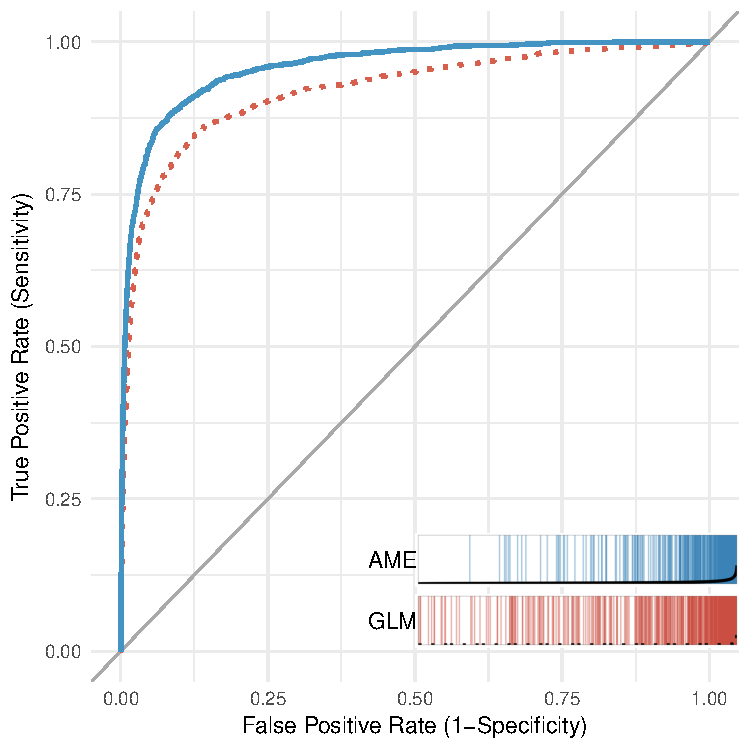
\includegraphics[width=.4\textwidth]{reiter_stam_roc_outSample.pdf} & 
		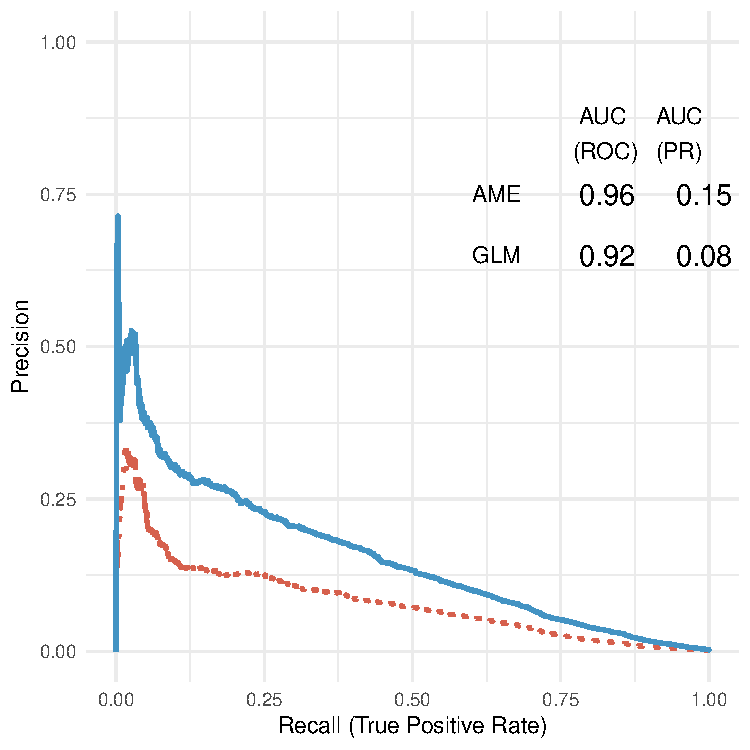
\includegraphics[width=.4\textwidth]{reiter_stam_pr_outSample.pdf} \\
		\multicolumn{2}{l}{\textbf{Weeks (2012)}} \\
		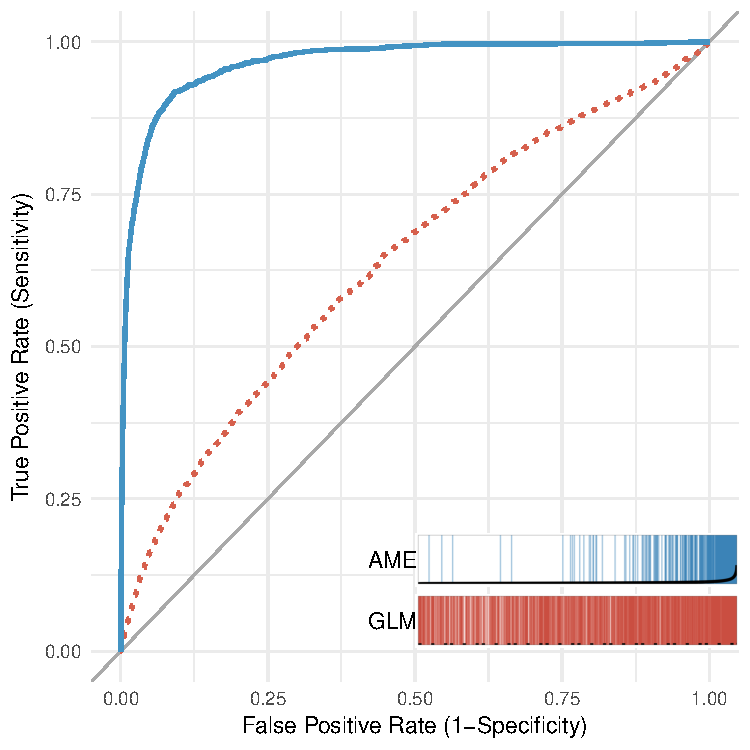
\includegraphics[width=.4\textwidth]{weeks_roc_outSample.pdf} & 
		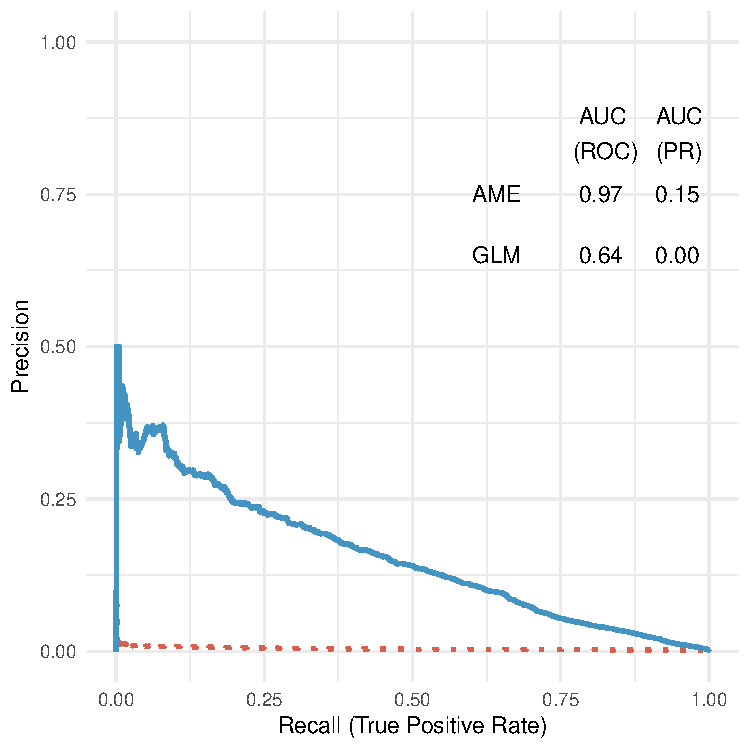
\includegraphics[width=.4\textwidth]{weeks_pr_outSample.pdf} \\
		\multicolumn{2}{l}{\textbf{Gibler (2017)}} \\
		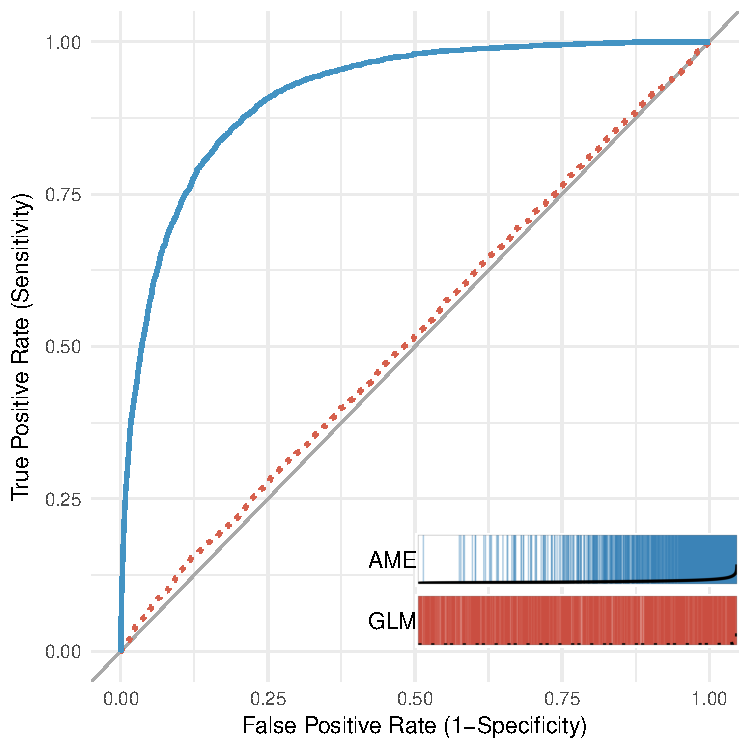
\includegraphics[width=.4\textwidth]{gibler_roc_outSample.pdf} & 
		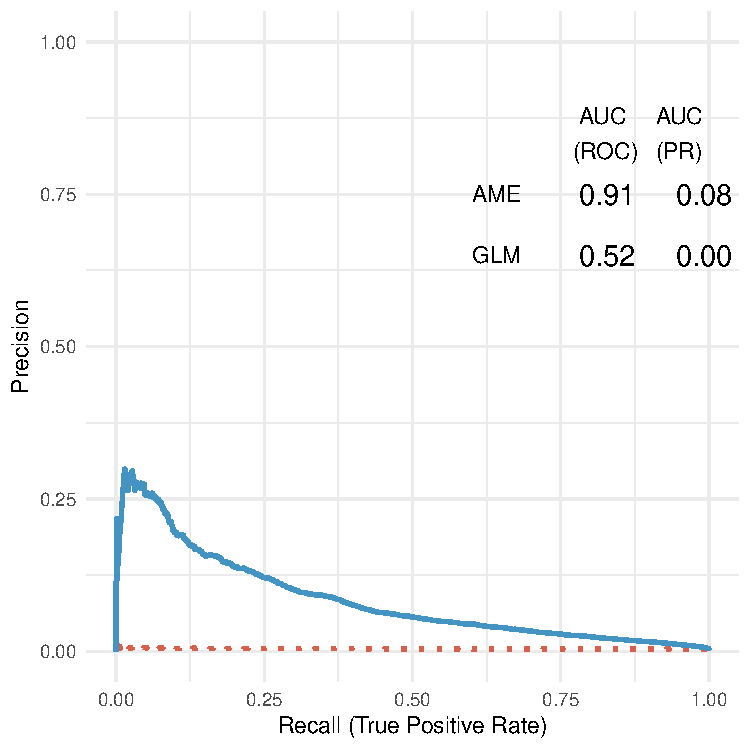
\includegraphics[width=.4\textwidth]{gibler_pr_outSample.pdf} \\
	\end{tabular}
	\caption{Assessments of out-of-sample predictive performance for Gibler (2017) using ROC curves, PR curves, and separation plots.}
	\label{fig:perf}	
\end{figure}

Each of the studies has a crucial finding that we hone in on to further draw into focus the analytical power of the AME estimation procedure.  In Table~\ref{tab:modelFindingSumm}, we present the overall results; the term \textit{Unconfirmed} indicates only that the sign and/or significance of the putatively crucial finding in the original study is not found to hold in the AME estimation.\footnote{Full tabular results for each of the original and reestimated models are presented in the Appendix.}

\begin{table}[ht]
\centering
\caption{Here we provide a brief summary of the key variable in each of the replications and a note about whether or not the highlighted finding remains when using our network-based approach.}
	\begin{tabular}{l p{7cm} l} \toprule
		\multirow{2}{*}{Study} & \multirow{2}{*}{Central Finding} &  Confirmed after \\
		& &  accounting for dependencies? \\ \toprule
		Reiter \& Stam (2003) & Personalist Regimes Attack Democracies, Not Vice Versa & {Confirmed} \\ \midrule
		Weeks (2012) & Bosses, Juntas, and Strongmen are more Aggressive, Machines are Not & {Unconfirmed} \\\midrule
		Gibler (2017) & Power Parity at Time of Entry to International System Increases Conflict & {Unconfirmed}\\ \bottomrule
	\end{tabular}
	\label{tab:modelFindingSumm}
\end{table}

An important takeaway here is that many scholars are forced to make knowledge claims based on the statistical significance of a small set of covariates, or the differences between these covariates. These differences may change dramatically when interdependencies are taken into account directly. This outcome follows from AME's ability to better account for the dependencies discussed in the previous section, whereas GLM approaches explicitly assume observational independence conditional on the specified covariates. As this is a widely-known limitation of GLM approaches, scholars often attempt to account for clustering of observations by including additional variables and adjusting the standard errors of the resulting estimates. At best, this method introduces noise and imprecision into results, and at worst can produce misleading outcomes. 

\subsection{....}

Apart from providing stronger inferential guarantees and predictive performance than conventional approaches, the AME framework 


reiter and stam take a look at the srm effeccts to understand where the model is still falling short

mcdonald we recover support fro trade dependenicence and also find eveidence for their highest barrier to trade variable

for weeks even though we dont find support for her hypothesis we do se esomething interesting in the multiplicative effects

for gibler 

